\documentclass[11pt]{article}
\usepackage[a4paper,margin=19mm]{geometry}
\usepackage{amsmath,booktabs,graphicx,hyperref,array}
\setlength{\parindent}{0pt}\setlength{\parskip}{6pt}\setlength{\emergencystretch}{2em}
\begin{document}
\begin{center}{\Large Groups represented by incidence geometries}\\[3pt]
Complete written comparison: two originals and one shared theory
\end{center}
The complete replacement is longer in the fixed primary measure:
\[
 \frac{c(\mathrm{F010})+c(\mathrm{L126})}{c(U)+c(R_1)+c(R_2)}
 =\frac{25\,348+35\,124}{36\,715+10\,985+34\,452}
 =\frac{60\,472}{82\,152}\approx\mathbf{@WRITTEN@}.
\]
\textbf{This is expansion, not achieved whole-topic compression.}
The whole common proof is paid once, including the finite-normal-pair
existence proof now shared by both applications. Neither application is
an uncharged prerequisite of its sibling.

The fixed primary coordinate is \emph{calibrated selected text, NFC,
characters excluding whitespace}. It preserves the prior F010 source
policy. All pages and references are included: two sources of 13 pages
each, common theory 13 pages, and applications of 4 and 12 pages.
Exact running furniture is removed and bound glyph aliases are applied;
raw, untrimmed text remains an explicit sensitivity.

\begin{center}\begin{tabular}{lrrr}\toprule
Conditional reuse & Source & Complete local paper & Factor\\\midrule
F010 after whole $U$ and premises &25\,348&10\,985&@F010@\\
L126 after whole $U$ and premises &35\,124&34\,452&@L126@\\\bottomrule
\end{tabular}\end{center}
These conditional factors describe reuse \emph{after} acquiring the
whole common theory and actual retained classical premises. L126 also
requires the complete graph certificate and graph JSON described on
page~2. The nine optional checks are not acquisition prerequisites.
Conditional reuse does not undo the growth of the complete shared proof.

\begin{center}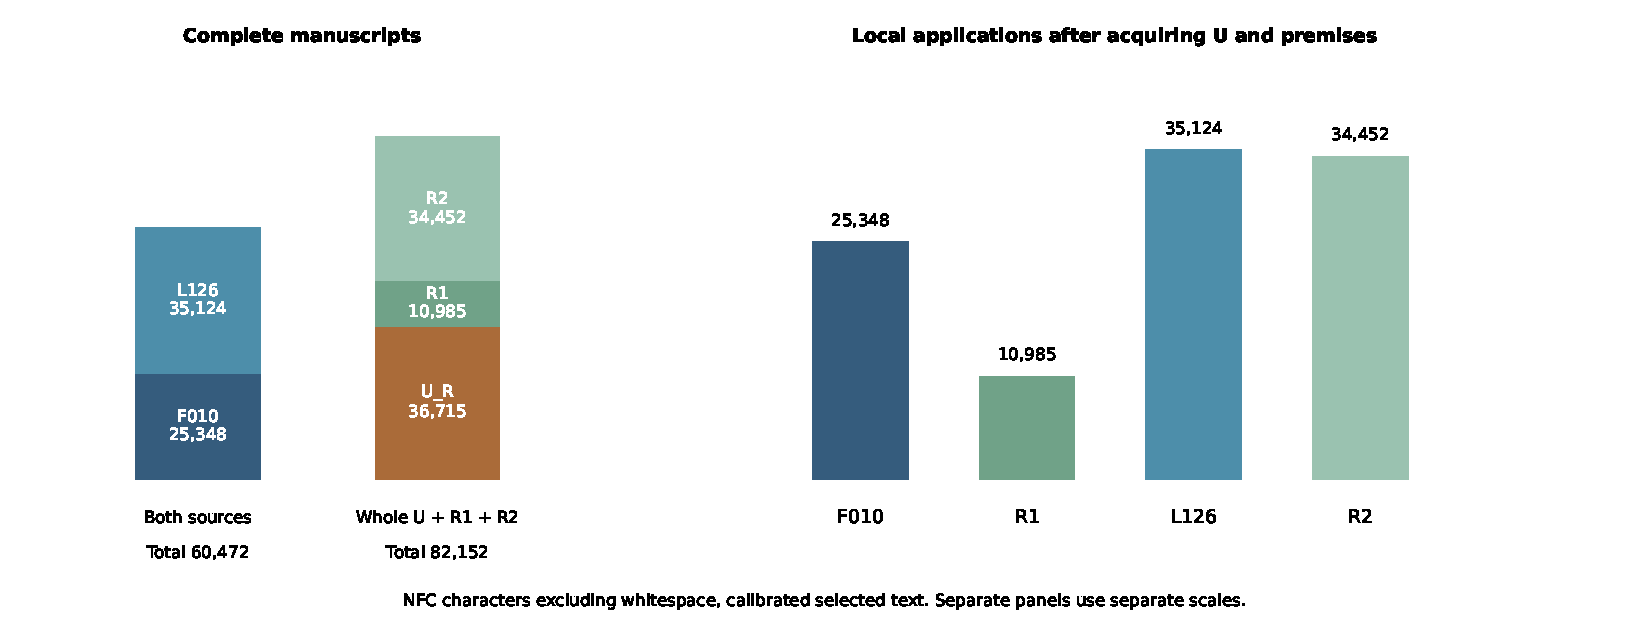
\includegraphics[width=\linewidth]{costs.pdf}\end{center}
\textbf{Scope of the numbers.} These are manuscript lengths, not minimal
proof lengths, mathematical difficulty, or total research effort.
Executable listings are excluded on both sides; written mathematical
algorithms and proofs remain. Software-inclusive factors are unknown,
not zero, because matched source software and all outside proof costs
are unavailable.

\newpage
\begin{center}{\Large What has to be acquired}\end{center}
\begin{center}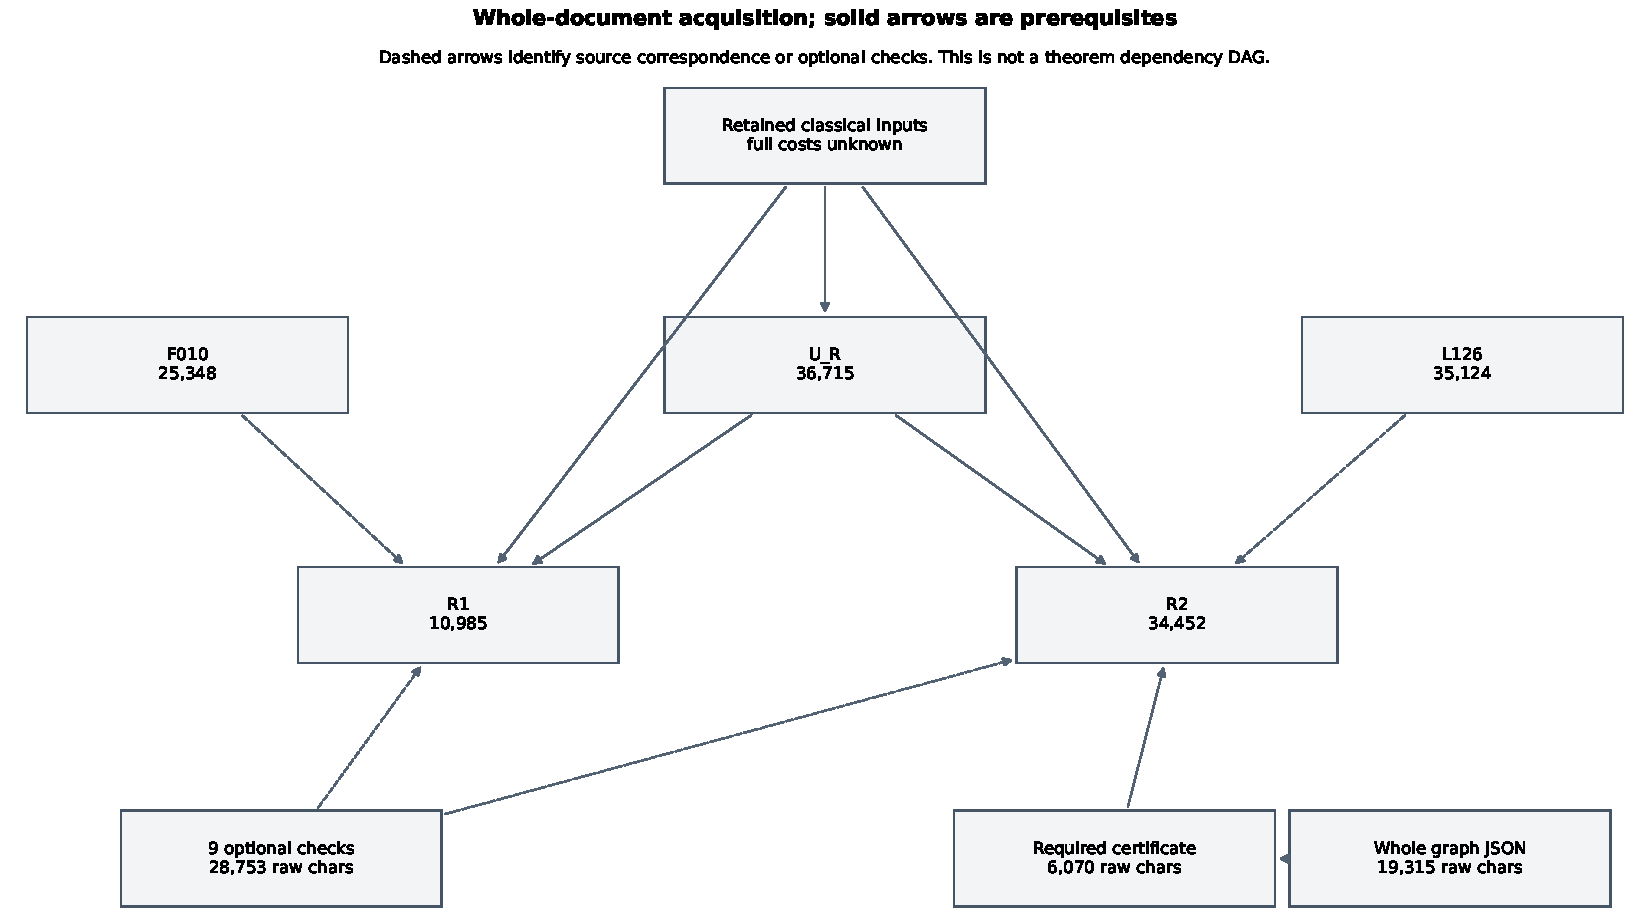
\includegraphics[width=\linewidth]{document_graph.pdf}\end{center}
The diagram shows whole-document acquisition and evidence association,
not an internal theorem dependency graph. Its box counts carry no
compression factor. Starting with the complete common paper costs
36\,715; adding all of $R_1$ reaches 47\,700; adding all of $R_2$
reaches 82\,152. All local context and bibliography are paid.

\textbf{Required finite premise for L126.} The complete
\texttt{certificate/check.py} is 8\,030 bytes (6\,070 primary raw
characters), and the full \texttt{certificate/graph.json} is
19\,326 bytes (19\,315 primary raw characters). The elementary
certificate establishes the full group of the 896-vertex graph used
in the Section~8 counterexample. Neither a summary nor the printed code
appendix substitutes for the complete graph data. These are actual
proof inputs even though manuscript ratios inventory their cost separately.

\textbf{Optional and separate evidence.} Nine complete validation
programs contain 35\,601 bytes (28\,753 primary raw characters).
The 16-page appendix prints all ten programs; its 35\,723 primary
characters and the ten raw programs' 34\,823 characters are alternative
representations, never added twice. The graph JSON remains separate.
Two orchestration helpers total 16\,622 bytes and four partial Lean files
15\,931 bytes. Their 22 declarations do not formalize either complete
source or the graph instance. Runtime, libraries, outside proofs and
full graphical structure retain unknown costs.

\newpage
\begin{center}{\Large Inventory, sensitivities and attribution}\end{center}
\begin{center}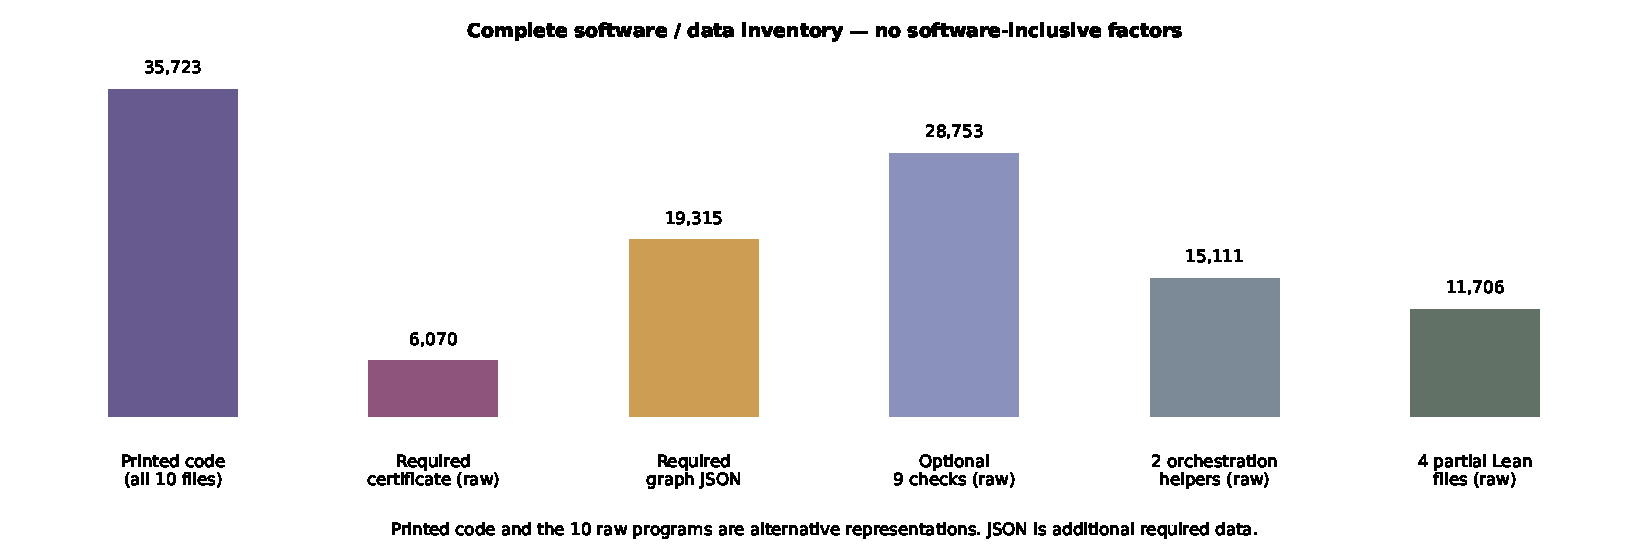
\includegraphics[width=\linewidth]{inventory.pdf}\end{center}
All 30 combinations of three text policies, NFC/NFKC and five units are
reported in \texttt{results.json}, with exactly 30 whole-written and
60 conditional fractions. The selected calibrated NFC slice is:
\begin{center}\begin{tabular}{lrrr}\toprule
Unit & Whole written & F010 conditional & L126 conditional\\\midrule
@SENSITIVITY@
\bottomrule\end{tabular}\end{center}
The complete old F010 source vector is unchanged. Every current
replacement PDF, including the changed four-page $R_1$, was newly
extracted in the accepted input packet. This numerical packet performs
no new extraction, font reconstruction, scientific computation or proof
review. No alternative unit is substituted for the fixed primary. The full raw,
untrimmed NFC nonspace coordinate gives @RAW@ for the whole comparison;
it is a sensitivity, not a replacement headline.

\textbf{Exact source boundary.} F010 is D\'iaz Ramos--Molinier--Viruel,
\emph{Every finite group is represented by a finite incidence geometry},
arXiv:2511.02410v2, 16 December 2025. L126 is Leemans--Stokes--Tranchida,
\emph{Groups represented by incidence geometries},
arXiv:2506.10464v1, June 2025. The accepted scientific contract retains
all six F010 blocks and 31 L126 dispositions, including explicit
finite-field and small-case corrections and the chamber-connectivity
qualification for splitting. The broader Section~6.2 and Section~8
programmes are not claimed solved. Classical projective, Tits, Frucht
and named-group premises remain attributed and unpriced.

\textbf{Review boundary.} The scientific successor, proof relocation
and input boundary have distinct accepted reviews. This author numerical
packet requires its own independent arithmetic and reader review.
It claims no new source, question, formalization or historical-priority
credit. Earlier frozen editions remain intact.
\end{document}
